\documentclass[letterpaper,10pt]{article}\usepackage[]{graphicx}\usepackage[]{color}
%% maxwidth is the original width if it is less than linewidth
%% otherwise use linewidth (to make sure the graphics do not exceed the margin)
\makeatletter
\def\maxwidth{ %
  \ifdim\Gin@nat@width>\linewidth
    \linewidth
  \else
    \Gin@nat@width
  \fi
}
\makeatother

\definecolor{fgcolor}{rgb}{0.345, 0.345, 0.345}
\newcommand{\hlnum}[1]{\textcolor[rgb]{0.686,0.059,0.569}{#1}}%
\newcommand{\hlstr}[1]{\textcolor[rgb]{0.192,0.494,0.8}{#1}}%
\newcommand{\hlcom}[1]{\textcolor[rgb]{0.678,0.584,0.686}{\textit{#1}}}%
\newcommand{\hlopt}[1]{\textcolor[rgb]{0,0,0}{#1}}%
\newcommand{\hlstd}[1]{\textcolor[rgb]{0.345,0.345,0.345}{#1}}%
\newcommand{\hlkwa}[1]{\textcolor[rgb]{0.161,0.373,0.58}{\textbf{#1}}}%
\newcommand{\hlkwb}[1]{\textcolor[rgb]{0.69,0.353,0.396}{#1}}%
\newcommand{\hlkwc}[1]{\textcolor[rgb]{0.333,0.667,0.333}{#1}}%
\newcommand{\hlkwd}[1]{\textcolor[rgb]{0.737,0.353,0.396}{\textbf{#1}}}%

\usepackage{framed}
\makeatletter
\newenvironment{kframe}{%
 \def\at@end@of@kframe{}%
 \ifinner\ifhmode%
  \def\at@end@of@kframe{\end{minipage}}%
  \begin{minipage}{\columnwidth}%
 \fi\fi%
 \def\FrameCommand##1{\hskip\@totalleftmargin \hskip-\fboxsep
 \colorbox{shadecolor}{##1}\hskip-\fboxsep
     % There is no \\@totalrightmargin, so:
     \hskip-\linewidth \hskip-\@totalleftmargin \hskip\columnwidth}%
 \MakeFramed {\advance\hsize-\width
   \@totalleftmargin\z@ \linewidth\hsize
   \@setminipage}}%
 {\par\unskip\endMakeFramed%
 \at@end@of@kframe}
\makeatother

\definecolor{shadecolor}{rgb}{.97, .97, .97}
\definecolor{messagecolor}{rgb}{0, 0, 0}
\definecolor{warningcolor}{rgb}{1, 0, 1}
\definecolor{errorcolor}{rgb}{1, 0, 0}
\newenvironment{knitrout}{}{} % an empty environment to be redefined in TeX

\usepackage{alltt}

\usepackage[left=0.75in, right=0.75in, top=0.75in, bottom=0.75in]{geometry}
\usepackage{longtable}
\usepackage{amsmath}
\usepackage{amssymb}
\usepackage{bm}

\newcommand{\question}[3]{
\begin{itemize}
\item[{\makebox[1cm]{#1)}}] #2

\vspace{.2in}

#3

\end{itemize}

\vspace{.2in}
}
\IfFileExists{upquote.sty}{\usepackage{upquote}}{}
\begin{document}

{\large Chapter 2 Homework}
\hfill
{\large Justace Clutter}

\vspace{.1in}

\hrule

\vspace{.5in}

\question{2.1}{
Show that $F=(S/N)_{\text{in}}/(S/N)_{\text{out}}=(N_\text{out}/N_\text{in})(S_\text{in}/S_\text{out})=(N_\text{out}/N_\text{in})(1/G_\text{LNA})$ if and only if $T_\text{ant}=T_\text{radar}=T_0$.
}{

Let's start be going backwards from the equations in the problem to show that that $F = (N_\text{out}/N_\text{in})(1/G_\text{LNA}) = (S/N)_{\text{in}}/(S/N)_{\text{out}}$.  

\begin{align*}
F & = \frac{N_\text{out}}{N_\text{in}G_\text{LNA}} \\
  & = \frac{N_\text{out}}{N_\text{in}\left(\frac{S_\text{out}}{S_\text{in}}\right)} \\
  & = \left(\frac{N_\text{out}}{N_\text{in}}\right)\left(\frac{S_\text{in}}{S_\text{out}}\right) \\
  & = \left(\frac{S_\text{in}}{N_\text{in}}\right)\left(\frac{N_\text{out}}{S_\text{out}}\right) \\
  & = \left.\left(\frac{S_\text{in}}{N_\text{in}}\right)\middle/\left(\frac{S_\text{out}}{N_\text{out}}\right)\right.
\end{align*}

In the strictest sense, the noise factor is the ratio of the noise out of a practicl amplifier, in this case the LNA, and the noise out of an ideal amplifier at the standard temperture $T_0=290$ K.  Up to this point there have been no assumptions on what the form of $N_\text{in}$ and $N_\text{out}$ were.  Using equation 2.10 from the text we can compose forms for $N_\text{in}$ and $N_\text{out}$.  Since the strict definiton of $F$ assumes an ideal amplifier, $N_1$.

In the above equations, there were no attempts to explain what $N_\text{in}$ and $N_\text{out}$ were and what they contained.  The noise factor is a property of the amplifier, in this case the LNA.  

In the first line of the solution, the core definition of the noise factor is used.  Namely, this is that the noise factor is equal to the ratio of the measured output noise to the noise that would be generated after the LNA assuming an overall system temperature of $T_0=290$ K.  


In this work there were no assumptions made on the input noise and it was simply denoted as $N_\text{in}$.  This noise represents the noise intorduced in the system up to the LNA which includes noise from the antenna and the radar itself.  

}

\question{2.2}{
Show that, if we define $F2=(S/N)_\text{in}/(S/N)_\text{out}$ and it $T_\text{ant}=T_\text{radar}$, then $T_\text{rcvr}=(F2-1)T_\text{ant}$.
}{}

\question{2.3}{
Consider a sensitive radar observing targets against deep space ($T_\text{ant}=3\text{K}$), with an LNA cooled with liquid helium to $T_\text{rcvr}=4.2\text{K}$.  If $L_\text{radar}=1$, what is the noise figure in decibels?  What is $T_\text{sys}$?
}{}

\question{2.4}{
In the front-end circuit shown in Figure 2.11, the designer has put a system gain control, in the form of a variable attenuator, after the first LNA.  Sketch the variation of overall system gain and system noise figure as this attenuator is varied over its full range. (Assume that $T_\text{ant}=T_\text{radar}=T_0$.)
}{}

\question{2.5}{
Show that the standard deviation of the quantization error and an A/D converter is

\begin{equation*}
\sigma_\epsilon = \frac{\text{\textit{least significant bit}}}{\sqrt{12}}
\end{equation*}
}{}

\question{2.6}{
Consider a spherical wave emitted from a point antenna.  For the far field, we want the wave to be essentially planar over an aperture of width D at range R.  If the far-field criterion is that the wavefront deviate no more than $\frac{\lambda}{16}$ from a plane (the Fraunhofer criterion), show that $R$ (far field) $= 2D^2/\lambda$.  Calculate the near- and far-field ``boundaries'' ($R=2D^2/\lambda$), for $D=1$m, at L, S, X, Ku, and Ka bands.
}{

The following solution depends on the small angle approximation:

\begin{equation*}
x = r\left(1-\frac{\theta^2}{2}\right) \qquad \text{ and } \qquad y = r\theta \text{.}
\end{equation*}

\begin{minipage}{3in}
\begin{center}
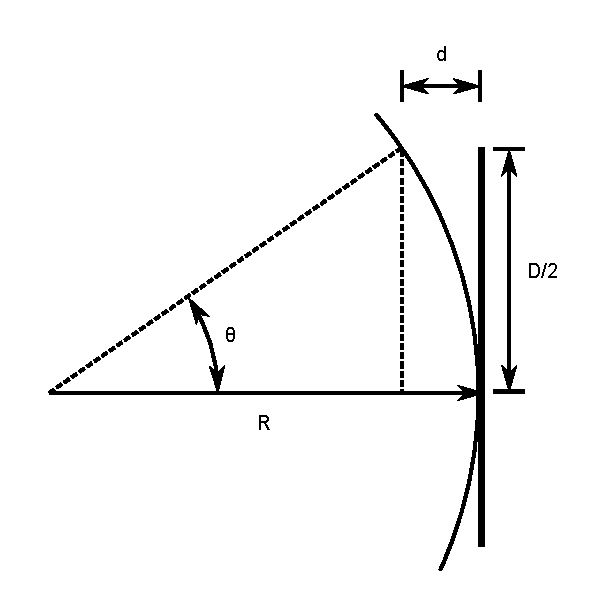
\includegraphics[width=3in]{Figures/HW2_2_6__1.pdf}
\end{center}
\end{minipage}
\begin{minipage}{3in}

\begin{align*}
y & = \left.R\theta\right|_{y=\frac{D}{2}} \rightarrow \theta = \frac{D}{2R} \\
\therefore x & = R\left(1-\frac{\left(\frac{D}{2R}\right)^2}{2}\right) \\
d & = R - x \\
& = R - R\left(1-\frac{\left(\frac{D}{2R}\right)^2}{2}\right) \\
\therefore R & = \frac{D^2}{8d}
\end{align*}
\end{minipage}

Evaluating the final equation for $R$ with the substitution that $d=\frac{\lambda}{16}$ yeilds the final relationship for the far-field threshold range:

\begin{equation*}
R = 2\frac{D^2}{\lambda}
\end{equation*}

\begin{knitrout}
\definecolor{shadecolor}{rgb}{0.969, 0.969, 0.969}\color{fgcolor}

{\centering 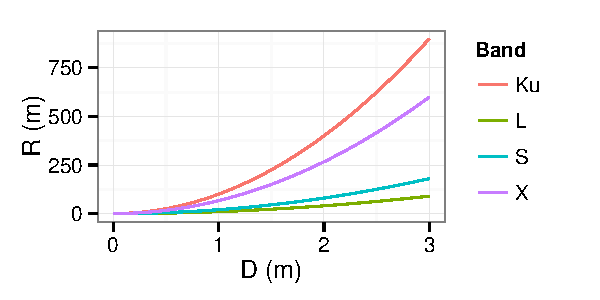
\includegraphics[width=\maxwidth]{figure/unnamed-chunk-1} 

}



\end{knitrout}

The threshold range for the far field for the L band, S Band, X Band, and Ku Band is 10 m, 20 m, 66.6667 m, 100 m, respectively.

}

\question{2.7}{
Using Huygen's principle, deriver Snell's law of refraction between two media: $n_1\sin\theta_1=n_2\sin\theta_2$, where $n$ is the index of refraction and $\theta$ is the incidence angle (zero for normal incidence).
}{}

\question{2.8}{
Calculate the coordinate-transform matricies between the $(\theta, \phi)$ coordinates and the $(\alpha, \epsilon)$ coordinates.  Suppose that $\alpha=-30$ degrees and $\epsilon=45$ degrees; find $\theta,\phi$.  Suppose that $\theta=45$ degrees and $\phi=30$ degrees; find $\alpha, \epsilon$.
}{}

\question{2.9}{
For an infinite slit aperture of width $L$ parallel to the $x$ axis, with $\boldsymbol{E}$ perpendicular to the slit edges --- $\boldsymbol{E}=(0, E_y, 0)$ --- in the $yz$ plane, show that $E_x=0$ and in the $yz$ plane, in polar coordinates,

\begin{equation*}
E_\theta(r, \theta) = jk\frac{e^{-jkr}}{2\pi r}E_yL\text{ sinc}\left(\frac{kL\sin\theta}{2}\right)
\end{equation*}
}{}

\question{2.10}{
For a finite rectangular aperture, $L_x$ by $L_y$, with $\boldsymbol{E}=\boldsymbol{E_0}$ parallel to $\boldsymbol{y}$, show that

\begin{align*}
E_\theta(r, \theta, \phi) & = jk\frac{e^{-jkr}}{2\pi r}E_0L_xL_y\sin\phi\text{ sinc}\left(\frac{kL_x}{2}\mu\right)\text{ sinc}\left(\frac{kL_y}{2}\nu\right) \\
E_\phi(r, \theta, \phi) & = jk\frac{e^{-jkr}}{2\pi r}E_0L_xL_y\cos\theta\cos\phi\text{ sinc}\left(\frac{kL_x}{2}\mu\right)\text{ sinc}\left(\frac{kL_y}{2}\nu\right)
\end{align*}

where $\mu=\sin\theta\cos\phi$, $\nu=\sin\theta\sin\phi$. (The underlined factors are the obliquity factos.)  In the $E$ plane ($yz$ plane), $\phi=90$ degrees; show that

\begin{equation*}
E_\theta(r,\theta) = jk\frac{e^{-jkr}}{2\pi r}E_0L_xL_y\text{ sinc}\left(\frac{kL_y}{2}\sin\theta\right), \quad E_\phi = 0
\end{equation*}

In the $H$ plane ($xz$ plane), $\phi=0$ degrees; show that

\begin{equation*}
E_\theta(r,\theta) = jk\frac{e^{-jkr}}{2\pi r}E_0L_xL_y\cos\theta\text{ sinc}\left(\frac{kL_x}{2}\sin\theta\right), \quad E_\phi = 0
\end{equation*}
}{}

\question{2.11}{
For a circular aperture of radius $a$, with $\boldsymbol{E}=\boldsymbol{E}_0$ parallel ro the aperture plane, show that

\begin{align*}
\boldsymbol{E} & = \left(\hat{\boldsymbol{\theta}}\cos\phi-\hat{\boldsymbol{\phi}}\sin\phi\cos\theta\right)jk\frac{e^{-jkr}}{2\pi r}\cdot \boldsymbol{E}_02\pi a^2\frac{J_1(ka\sin\theta)}{ka\sin\theta} \\
f(\theta,\phi) & = f_1(\theta) = \frac{2J_1(ka\sin\theta)}{ka\sin\theta}
\end{align*}
}{}

\question{2.12}{
Show that for the infinite slit and its characteristic $\sin(x)/x\equiv \text{sinc}(x)$ pattern, the first sidelobe peak is -13.3 dB below the mainlobe peak; show that for the circular aperture, the first sidelobe peak is -17.6 dB below the mainlobe peak.
}{}

\question{2.13}{
From the fundamental properties of a parabola, show that for a parabolic dish antenna with a point-source feed at the focal point and the aperture (planer surfece within rim of dish) perpendicular to the axis of revolution, all radiation leaving the aperture has the same phase.
}{

The parabola is constructed such that the distance between any point on the curve and the focal point is the same as the distance between that same point and what is called the directex.  This is represented mathematically as

\begin{equation*}
|y+b| = \sqrt{x^2 + (y-b)^2}\text{.}
\end{equation*}

In the figure below, the directex is the horizonatl dashed line below the $x$-axis and the above equation allows one state that the line segments $\overline{BF}$ and $\overline{BE}$ are the same length and that the line segments $\overline{CF}$ and $\overline{CD}$ are the same length.

\begin{center}
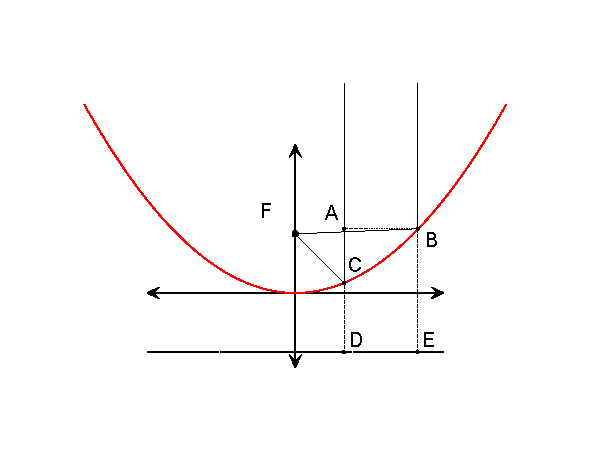
\includegraphics[width=4in]{Figures/HW2_2_13__1.pdf}
\end{center}

\begin{align*}
\overline{AD} & = \overline{BE} & \\
\overline{AD} & = \overline{BF} & \text{ Prop. of Parabola} \\
\overline{AC} + \overline{CD} & = \overline{BF} & \text{ Substitution} \\
\overline{AC} + \overline{CF} & = \overline{BF} & \text{ Prop. of Parabola} \\
\overline{ACF} & = \overline{BF} & \\
\end{align*}

Since the line segments $\overline{ACF}$ and $\overline{BF}$ are the same length, the phase of the signals will be the same as the signal leaves the antenna.


}

\question{2.14}{
For an axially symmetric parabolic reflector with a feed at the focus radiating isotropically with power $P$ a distance $d$ from the cloasest point on the reflector surface, show that the aperture illumination function $F(r)$ (W/m$^2$) is

\begin{equation*}
F(r) = \frac{P}{4\pi d^2}\cdot\frac{1}{\left(1+\frac{r^2}{4d^2}\right)^2}
\end{equation*}
}{}

\question{2.15}{
Shwo that, for an ideal rectuangular or circular aperture where $\lambda >>$ aperture dimension, the sidelobe envelope (smooth line connecting the sidelobe peaks), measured in dBi, is independant of $\lambda$ or the aperture dimension.  (The Internaional Radio Consultative Committee [CCIR] recommends that sidelobes for large circular apertures [D $> 100\lambda$] be below $G=29-25\log_{10}(\theta_\text{degrees})$ dBi [27].)
}{}

\question{2.16}{
Consider a long ($N >> 1$) linear array of length $L$.  Suppose that the conter $N/4$ elements burn out.  Develop a revised expression for the radiation pattern, for the mainlobe at 90 degrees (broadside), 45 degrees, and 0 degrees (endfire).
}{}

\question{2.17}{
Show that 


\begin{itemize}
\renewcommand{\labelitemi}{$\bullet$}
\item $kd < \pi \Rightarrow d < \lambda / 2$ (no grating lode occurs);
\item $\pi < kd < 2\pi \Rightarrow \lambda / 2 < d < \lambda$ (a grating lobe may occur);
\item $kd > 2\pi\Rightarrow d> \lambda$ (one of more grating lobes occur).
\end{itemize}

}{}

\question{2.18}{
Show that the criterion for no grating lobes (peak) is

\begin{equation*}
\frac{d}{\lambda}=\frac{1}{1+|\cos\theta|}
\end{equation*}

}{}

\question{2.19}{
If $\theta$ (mainlobe) $=30$ degrees, at what element spacing $(d/\lambda)$ do the peaks of the first, second, and thirdgrating lobes appear?
}{}


\end{document}
